\section{Parcial 2}
\begin{itemize}
    \item Planos tangentes y aproximaciones lineales 
    \item Regla de la cadena 
    \item Derivación implícita 
    \item Derivada direccional o razón de cambio en $f$ en la dirección de $\vec{u}$
\end{itemize}

\section{14.7 Máximos y mínimos}
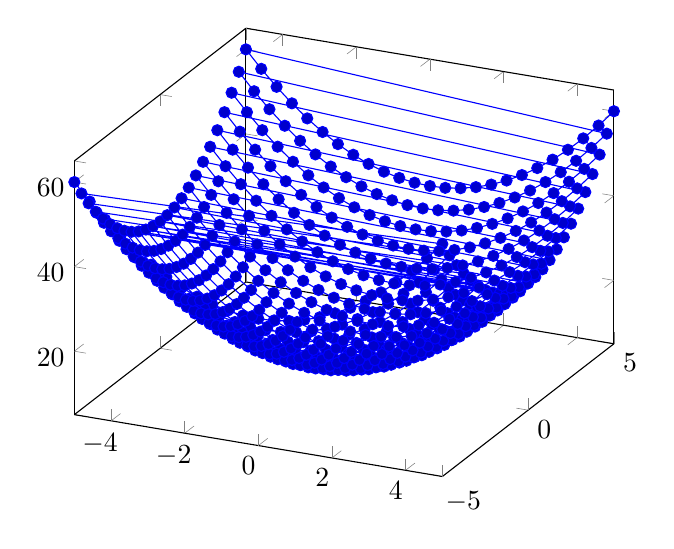
\begin{tikzpicture}
    \begin{axis}[mark=none]
        \addplot3{x^2 + y^2 + 10}; 
    \end{axis}    
\end{tikzpicture}

\begin{itemize}
    \item Máximo relativo:
        \begin{itemize}
            \item $\displaystyle f(a,b) > f(x,y)$
            \item $(x,v)$ cerca de $(a,b)$
        \end{itemize}   

    
    \item Mínimo relativo:
        \begin{itemize}
            \item $\displaystyle f(a,b) < f(x,y)$
            \item $(x,y)$ cerca de $(a,b)$
        \end{itemize}
\end{itemize}

\subsection{En funciones de una variable}
\begin{itemize}
    \item Números críticos: $\displaystyle f'(c)=0$ ó $\displaystyle f'(c) = \text{ indef}.$
    \item 2da derivada: 
        \begin{center}
            \begin{align*}
                f'(c) < 0 \qquad \text{ Máximo relativo } \\ 
                f'(c) > 0 \qquad \text{ Mínimo relativo } \\ 
                f'(c) = 0 \qquad \text{ Inconcluso } \\ 
            \end{align*}
        \end{center}
\end{itemize}

\subsection{En funciones de dos variables}
\begin{itemize}
    \item Puntos críticos:
        \begin{center}
           \begin{align*}
               f_x(a,b) = 0 \qquad \text{ \& } \qquad f_y(a,b)=0 \\ 
           \end{align*}
        \end{center}
    
    \item No es suficiente:
        \begin{center}
           \begin{align*}
               f_{xx} < 0 \qquad \text{ \& } f_{yy} < 0 \qq \text{ Máx relativo } \\ 
               f_{xx} > 0 \qquad \text{ \& } f_{yy} > 0 \qq \text{ Mín relativo }\\ 
           \end{align*}
        \end{center}
    
    \item Prueba de la segunda derivada: $(a,b)$ es un punto crítico y $f(x,y)$ tiene segundas derivadas continuas.
        \begin{center}
           \begin{align*}
               D(a,b) = \begin{vmatrix}
                   f_{xx} & f_{xy} \\ 
                   f_{yx} & f_{yy} \\ 
               \end{vmatrix} = f_{xx}f_{yy} - \p{f_{xy}}^2 \\  
           \end{align*}
        \end{center}
    
    \item Entonces:
        \begin{itemize}
            \item Máximo relativo: $D(a,b) > 0$ \& $f_{xx} < 0 $
            \item Mínimo relativo: $D(a,b) > 0$ \& $f_{xx} > 0 $
            \item Punto de silla: $D(a,b) < 0$ no hay ni mínimo ni máximo.
            \item Inconcluso: $D(a,b)=0$
        \end{itemize}
    
    \item Ejemplo: Considere la función $z=x^2+y^2$.
        \begin{itemize}
            \item Puntos críticos:
                \begin{center}
                   \begin{align*}
                       \begin{matrix}
                            z_x=2x=0 \\ 
                            z_y = -2y = 0 \\  
                       \end{matrix} 
                       \\ 
                       \text{ Prueba de la segunda derivada } \\ 
                       \begin{vmatrix}
                           2 & 000 \\ 
                       \end{vmatrix} \\ 
                   \end{align*}
                \end{center}
        \end{itemize}
\end{itemize}

\subsection{Ejercicios máximos y mínimos}
\begin{enumerate}
    \item Encuentre los máximos y mínimos relativos de las siguientes funciones.
        \begin{itemize}
            \item $\displaystyle f(x,y) = x^2+4y^2-6x+16y$ 
                \begin{center}
                   \begin{align*}
                        \begin{rcases}
                            f_x=2x-6=0 \implies x=3 \\ 
                            f_y = 8y+16 = 0 \implies y = -2 \\
                        \end{rcases}  \text{ Único punto crítico en: } \qq (3,-2) \\ 
                        D(x,y) = \begin{vmatrix}
                            f_{xx} & f_{xy} \\ 
                            f_{xy} & f_{zz} \\ 
                        \end{vmatrix} = \begin{vmatrix}
                            2 & 0 \\ 
                            0 & 8 \\ 
                        \end{vmatrix} = 16 \qq 16 > 0 \\ 
                        f_{xx} = 2 \qq 2>0 \\ 
                        \text{ Valor mínimo }: \qq f(3,-2) = -25 \\ 
                   \end{align*}
                \end{center}
            
            \item $\displaystyle g(x,y) = 2x^2+xy+y^2+100$ 
                \begin{center}
                   \begin{align*}
                       g_x = 4x+4 = 0 \qq \implies \qq y = -4x \qq implies y=0\\ 
                       g_y = x + 2y = 0 \qq implies \qq x-8x=-9x=0 \qq implies \qq x=0\\ 
                       \text{ \#Resolver ecuaciones } \\ 
                        \text{ Único punto crítico } \\ 
                        D(x,y) = \begin{vmatrix}
                            g_{xx} & g_{xy} \\ 
                            g_{yx} & g_{yy} \\ 
                        \end{vmatrix} = \begin{vmatrix}
                            4 & 1 \\ 
                            1 & 2 \\ 
                        \end{vmatrix} = 8-1 = 7 \qq \implies 7 > 0 \\ 
                        g_{xx} = 4>0 \\ 
                        \\
                        \text{ Valor mínimo relativo:  } \\ 
                        g(0,0) = 100 \\ 
                   \end{align*}
                \end{center}
            
            \item $\displaystyle h(x,y)=30-x^2-2y^2+4x-12y$ 
                \begin{center}
                   \begin{align*}
                        \begin{rcases}
                            \text{ Encontrar pts. críticos }: \qq h_x = 2x-4 = 0 \\ 
                            \text{ Encontrar pts. críticos }: \qq h_y = -4y-12 = 0 \\
                        \end{rcases} 
                        x = -\frac{4}{2} = 2 \\ 
                        y = \frac{12}{-4} = -3 \\ 
                        \text{ Único número crítico es (2,-3) }\\ 
                        D(x,y) = \begin{vmatrix}
                            -2 & 0 \\ 
                            0 & -4 \\ 
                        \end{vmatrix} = 8 > 0 
                        \qq \qq h_{xx} = -2 < 0 \\ 
                        \text{ Máximo relativo en (2,-3) } \; 38 \\ 
                   \end{align*}
                \end{center}
        \end{itemize}
    
    \item Una caja de cartón sin tapa, debe de tener un volúmen de $\displaystyle 32,000 cm^3$, calcule las dimensiones $\displaystyle x,y,z$  que minimicen el cartón utilizado.
        \begin{center}
           \begin{align*}
               \text{ Volúmen: } \qq V = xyz = 32,000 \\ 
               \text{ Área: } \qq A = 2zy+2zx+xy \\ 
               \text{ Tengo que minimizar el área } \\ 
               A = 2zy+2zx+xy \qq \implies \qq z = \frac{32,000}{xy}  \\ 
               x,y,z > 0 \\
               A(x,y) = 64,000 \cdot \frac{y}{xy} + 64,000 \frac{x}{xy} + xy \\ 
               A(x,y) = \frac{64,000}{x^2} + \frac{64,000}{y}   + xy \\ 
               A_x = 0 : \qq \frac{-64,000}{x^2} + y = 0 \qq \implies  \qq y = 64,000x^{-2} \\ 
               A_y = 0 : \qq \frac{-64,000}{y^2} +x = 0 \qq  \implies \qq [64,000]^2x^{-4} \\ 
               \text{ Sustituya en Ay } \qq \frac{-64,000}{(64,000)^2x^{-4}} + x = 0 \\ 
               -\frac{x^4}{64,000}  = -x \\ 
               x = \sqrt[3]{64} \cdot \sqrt[3]{1,000} = 4 \cdot 10 = 40 \\ 
               y = \frac{64,000}{x^2} = \frac{64 \cdot 1,000}{16 \cdot 100} = 4\cdot 10 = 40  \\ 
               z = \frac{32,000}{40 \cdot 40 } = \frac{32,000}{16,000} = 20 \\ 
               \therefore \; \text{ Las dimensiones que minimizan el área es:  } \qq x = y = 40 ,\qq z = 20 \\  
           \end{align*}
        \end{center}
    
    \item Discriminación de precios: 
        \begin{itemize}
            \item Demanda:
                \[
                    \begin{rcases}
                        \begin{matrix}
                            p_1 = 104-q_1 \\ 
                            p_2 = 84-q_2 \\ 
                        \end{matrix} \text{ Producción:  }\; q_1, q_2 
                    \end{rcases}
                \]
            
            \item Costos: 
                    \[
                      C = 600 + 4q_1 + 4q_2
                    \]
            
            \item Encuentre los precios y las cantidades $\displaystyle q_1$ \& $\displaystyle q_2$ a la que deben venderse los productos para maximizar la utilidad.
        \end{itemize}
        \begin{center}
           \begin{align*}
               \text{ Utilidad } = \text{ Ingresos } - \text{ Costos } \\ 
               \text{ Utilidad }: \qq u(q_1,q_2) = p_1q_1 + p_2q_2-600-4_q1-4q_2 \\ 
               u(q_1,q_2) = 104q_1 - q_1^2 + 84q_2 - q_2^2-600-4q_1-4q_2 \\ 
               u(q_1,q_2) = -q_1^2 - q_2^2 + 100q_1 + 80q_2 - 600 \\ 
               \dervpar{u}{q_1} = -2q_1 +100 = 0 \qq \implies  \qq q_1 = 50  \\ 
               \dervpar{u}{q_2} = -2q_2+80 = 0 \qq \implies  \qq  q_2 = 40 \\ 
               \text{ Único punto crítico:  } \qq \p{q_1=50, q_2=40} \\ 
               \begin{rcases}
                   q_1 = 50 \implies p_1 = 40 \\ 
                   q_2 = 40 \implies p_2 = 44 \\ 
               \end{rcases} \text{ discriminación } \\ 
               \text{ Utilidad máxima:  } \qq u(50,40) = 54\cdot 50 + 44 \cdot 40 - 600 - 360 \\ 
               2,700 + 1,760 - 960 = 35,00 \; \qq \text{ utilidad máxima } \\ 
               \text{ Prueba de la segunda derivada }: \\ 
               D(x,y) = \begin{vmatrix}
                   -2 & 0 \\ 
                   0 & -2 \\ 
               \end{vmatrix} = 4 > 0 \\ 
               v_{q_1q_1} = -2 <0 \\ 
           \end{align*}
        \end{center}
\end{enumerate}

